\section{Experiment}
\label{sec:experiment}
We will start by showing some results demonstrating forgetting in simple networks on a simple dataset, MNIST and split-MNIST, before moving onto our results on the CIFAR10 and split-CIFAR10 datasets using our more complex networks. 

\subsection{Demonstrating Forgetting}
\label{sec:demo_forgetting}
In this section we will demonstrate forgetting in simple networks, the FCFFNN and the CNN, on a simple dataset, MNIST. First we trained the networks in the \textbf{batch scenario on MNIST}, to gauge the kind of performance we should expect from these models on split-MNIST, the training and testing accuracy over training is shown in \cref{fig:MNIST-Batch-acc}. We clearly see an increase in accuracy over training, with the CNN achieving a final testing accuracy of 98.55\% and the FCFFNN achieving a final testing accuracy of 97.19\%, which is a good level of performance. Observing \cref{fig:MNIST-Batch-loss} we also note that the loss is doing what we might expect; which is it decreases very quickly at first followed by a continual gradual decrease. Note that we had to run training on the FCFFNN for 50 more epochs than we trained the CNN to achieve the performance stated. The models that produced these results were selected after trying out a number of different values for the learning rates which ended up at 0.005 for the CNN and 0.007 for the FCFFNN. We also tried out different values for the batch size, but found that the default value of 64 worked best for both models. 

We then trained these models in the \textbf{CL scenario on split-MNIST} (with 5 tasks) in the task-incremental setup. There was no modification to the networks, we used the same learning rate and batch size as in the batch setting. We sequentially trained the networks on each task and trained the networks on each task for 10 epochs. \Cref{fig:MNIST-CL-CTA} shows the CTAs obtained by the networks over training, we see that the CTA does decrease significantly when switching tasks (although this decrease is small in absolute amount), but that it increases to a very high accuracy by the end of training on the task. In fact, they achieve even better performance than in the batch scenario, although this is what we might expect due to the much simpler binary classification task that the network has to perform in the CL scenario. \Cref{fig:MNIST-CL-CTL} shows the loss obtained by the networks over training, this shows large spikes whenever training on new tasks begins which is what we might expect due to the new task containing different data, over the course of training on the task the loss then reduces. This indicates that both networks are successfully learning the new tasks when training on them and by the end of training have learnt the task proficiently.

\Cref{fig:MNIST-CL-TA} shows the training and testing accuracy each network achieved on each task over training, these plots confirm that the networks are learning the tasks well when training on them with the accuracy jumping very high. However, once the network moves onto learning a new task the accuracy on the previous task plummets very quickly. This decreased performance on the previous task is the network forgetting the previous task, we are therefore witnessing here the problem of CF. Note that the forgetting in these plots is very drastic with complete forgetting occurring after just one epoch of training on the next task with high frequency. Although we note that for some tasks, such as tasks 1 and 2 in experiments with the CNN, that complete forgetting doesn't occur until training begins on the next task. \Cref{fig:MNIST-CL-TL} shows the loss each network achieved on each task over training, we see the loss of the current task being trained drop significantly during training, but after or before training on the task its loss is gradually increasing. This collection of plots illustrates very clearly the problem of CF in two different networks on one of the "easiest" CL benchmarks (split-MNIST in the task incremental scenario). 


\begin{figure}[htbp]
    \centering
    \begin{subfigure}[t]{0.45\linewidth}
      \centering
      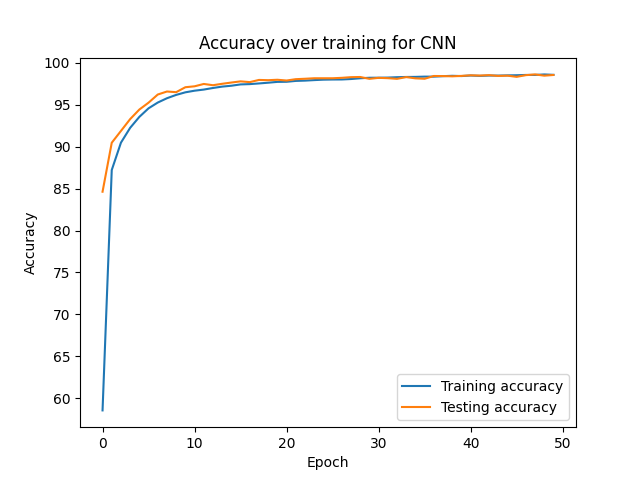
\includegraphics[width=\textwidth]{images/MNIST/CNN_acc.png}
      \caption{Accuracy over training epochs for the CNN on MNIST in the batch scenario. The final testing accuracy it achieved was 98.55\%.}
      \label{fig:MNIST-Batch-CNN-acc}
    \end{subfigure}
    \hspace{0.5cm}
    \begin{subfigure}[t]{0.45\linewidth}
      \centering
      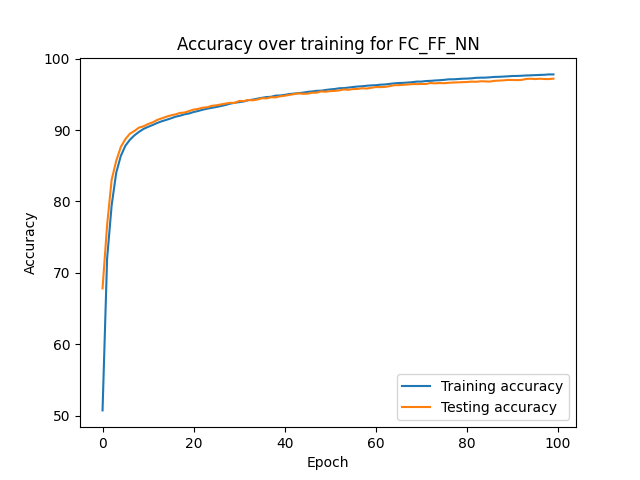
\includegraphics[width=\textwidth]{images/MNIST/FC_FF_NN_acc.png}
      \caption{Accuracy over training epochs for the FCFFNN on MNIST in the batch scenario. The final testing accuracy it achieved was 97.19\%.}
      \label{fig:MNIST-Batch-FCFFNN-acc}
    \end{subfigure}
    \caption{Accuracy over training on MNIST}
    \label{fig:MNIST-Batch-acc}
\end{figure}

\begin{figure}[htbp]
    \centering
    \begin{subfigure}[t]{0.45\linewidth}
      \centering
      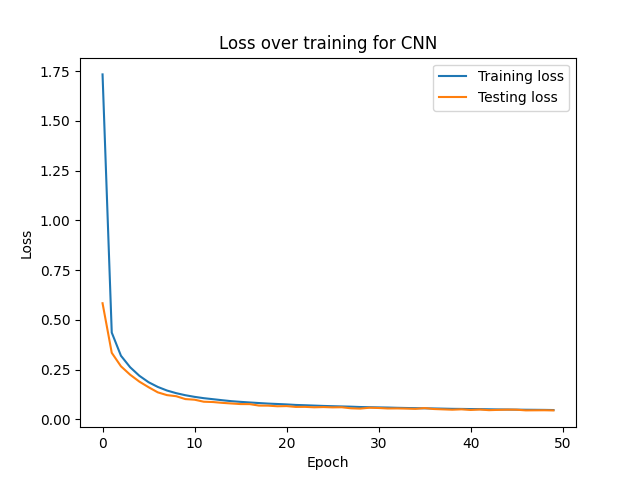
\includegraphics[width=\textwidth]{images/MNIST/CNN_loss.png}
      \caption{Loss over training epochs for the CNN on MNIST in the batch scenario. The final testing loss achieved was 0.0450 (3 sf.).}
      \label{fig:MNIST-Batch-CNN-loss}
    \end{subfigure}
    \hspace{0.5cm}
    \begin{subfigure}[t]{0.45\linewidth}
      \centering
      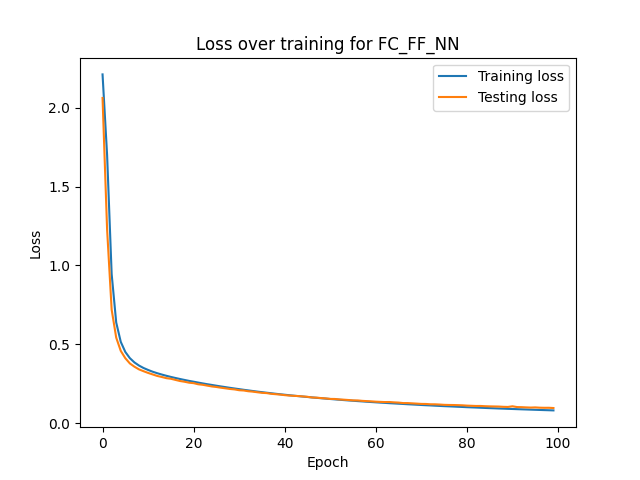
\includegraphics[width=\textwidth]{images/MNIST/FC_FF_NN_loss.png}
      \caption{Loss over training for the FCFFNN on MNIST in the batch scenario. The final testing loss achieved was 0.0956 (3 sf.).}
      \label{fig:MNIST-Batch-FCFFNN-loss}
    \end{subfigure}
    \caption{Cross entropy loss over training on MNIST}
    \label{fig:MNIST-Batch-loss}
\end{figure}

\begin{figure}[htbp]
    \centering
    \begin{subfigure}[t]{0.45\linewidth}
      \centering
      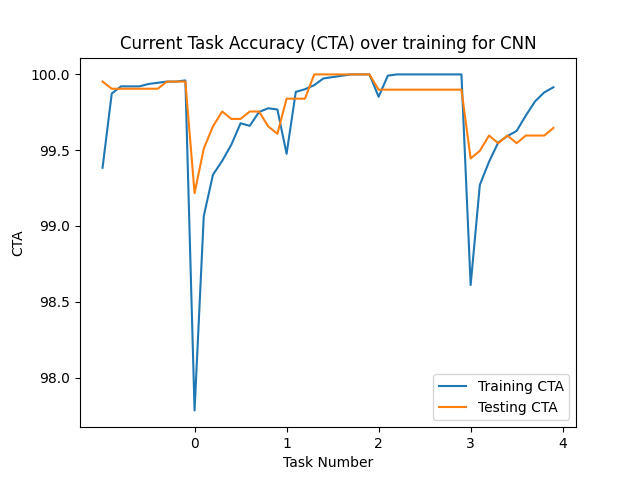
\includegraphics[width=\textwidth]{images/MNIST_CL/CNN_CTA.png}
      \caption{Current task accuracy over training epochs for the CNN on split-MNIST. It achieved the following test accuracies (on the current task) at the end of training on each task: Task 0 - 99.95\%, Task 1 - 99.61\%, Task 2 - 100\%, Task 3 - 99.9\%, Task 4 - 99.65\%.}
      \label{fig:MNIST-CL-CNN-CTA}
    \end{subfigure}
    \hspace{0.5cm}
    \begin{subfigure}[t]{0.45\linewidth}
      \centering
      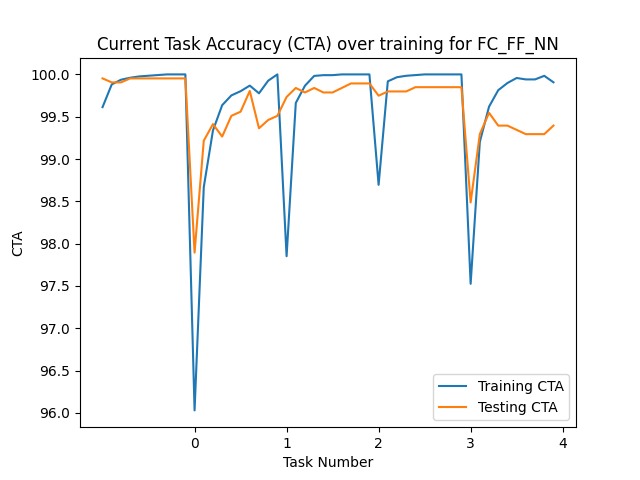
\includegraphics[width=\textwidth]{images/MNIST_CL/FC_FF_NN_CTA.png}
      \caption{Current task accuracy over training epochs for the FCFFNN on split-MNIST. It achieved the following test accuracies (on the current task) at the end of training on each task: Task 0 - 99.95\%, Task 1 - 99.51\%, Task 2 - 99.89\%, Task 3 - 99.85\%, Task 4 - 99.39\%.}
      \label{fig:MNIST-CL-FCFFNN-CTA}
    \end{subfigure}
    \caption{Accuracy over training on split-MNIST}
    \label{fig:MNIST-CL-CTA}
\end{figure}

\begin{figure}[htbp]
    \centering
    \begin{subfigure}[t]{0.45\linewidth}
      \centering
      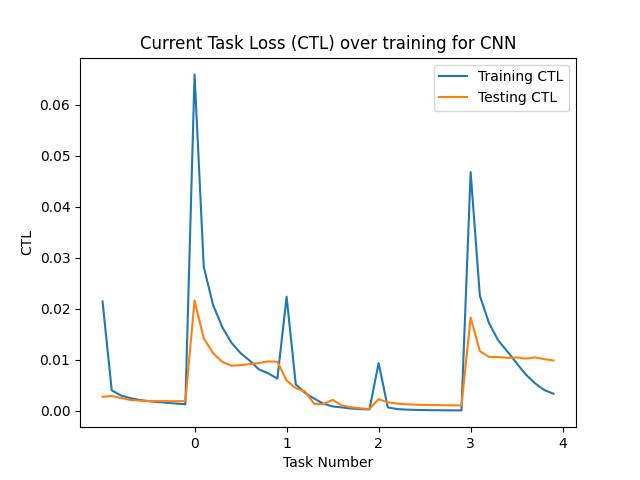
\includegraphics[width=\textwidth]{images/MNIST_CL/CNN_CTL.png}
      \caption{Current task loss over training epochs for the CNN on split-MNIST.}
      \label{fig:MNIST-CL-CNN-CTL}
    \end{subfigure}
    \hspace{0.5cm}
    \begin{subfigure}[t]{0.45\linewidth}
      \centering
      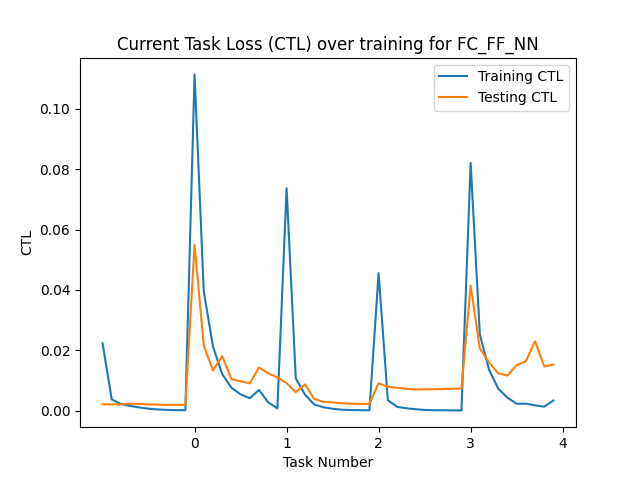
\includegraphics[width=\textwidth]{images/MNIST_CL/FC_FF_NN_CTL.png}
      \caption{Current task loss over training epochs for the FCFFNN on split-MNIST.}
      \label{fig:MNIST-CL-FCFFNN-CTL}
    \end{subfigure}
    \caption{Accuracy over training on split-MNIST}
    \label{fig:MNIST-CL-CTL}
\end{figure}

\begin{figure}[htbp]
    \centering
    \begin{subfigure}[t]{0.45\linewidth}
      \centering
      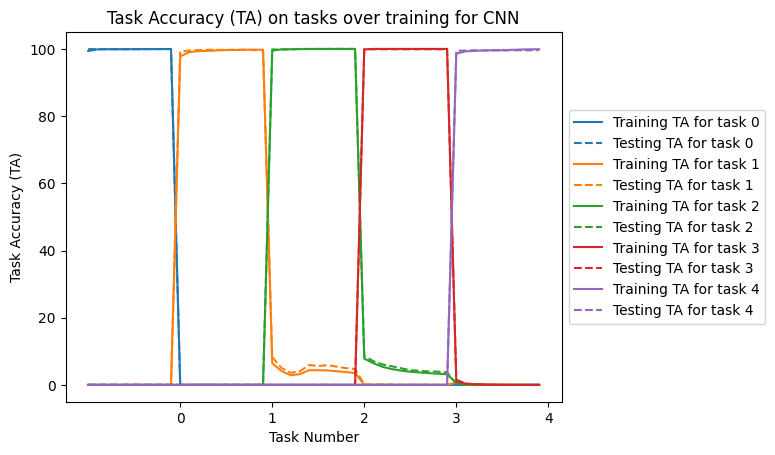
\includegraphics[width=\textwidth]{images/MNIST_CL/CNN_TA_task.png}
      \caption{Task accuracy on each task over training epochs for the CNN on split-MNIST. After training has finished on each task and training begins on the next the accuracy immediately falls to practically zero and stays there, except for task 1 and task 2 where the accuracy hovered around 4\%.}
      \label{fig:MNIST-CL-CNN-TA}
    \end{subfigure}
    \hspace{0.5cm}
    \begin{subfigure}[t]{0.45\linewidth}
      \centering
      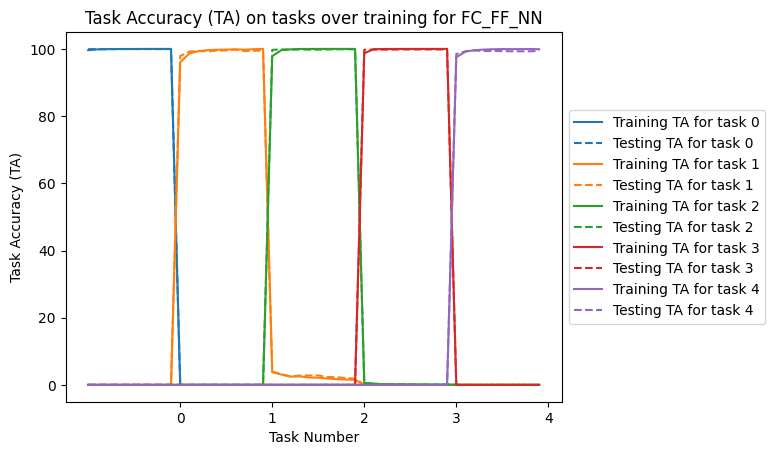
\includegraphics[width=\textwidth]{images/MNIST_CL/FC_FF_NN_TA_task.png}
      \caption{Task accuracy on each task over training epochs for the FCFFNN on split-MNIST. After training has finished on each task and training begins on the next the accuracy immediately falls to practically zero and stays there, except for after training on task 1 where the accuracy hovers around 3\%.}
      \label{fig:MNIST-CL-FCFFNN-TA}
    \end{subfigure}
    \caption{Accuracy over training on split-MNIST}
    \label{fig:MNIST-CL-TA}
\end{figure}

\begin{figure}[htbp]
    \centering
    \begin{subfigure}[t]{0.45\linewidth}
      \centering
      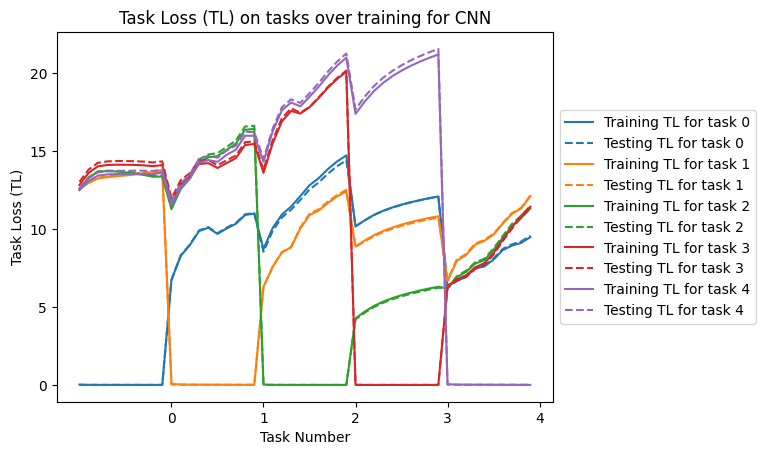
\includegraphics[width=\textwidth]{images/MNIST_CL/CNN_TL_task.png}
      \caption{Task loss on each task over training epochs for the CNN on split-MNIST.}
      \label{fig:MNIST-CL-CNN-TL}
    \end{subfigure}
    \hspace{0.5cm}
    \begin{subfigure}[t]{0.45\linewidth}
      \centering
      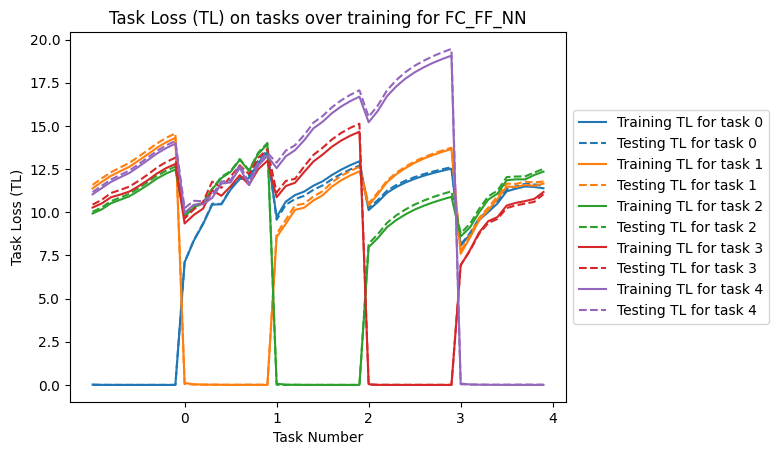
\includegraphics[width=\textwidth]{images/MNIST_CL/FC_FF_NN_TL_task.png}
      \caption{Task loss on each task over training epochs for the FCFFNN on split-MNIST.}
      \label{fig:MNIST-CL-FCFFNN-TL}
    \end{subfigure}
    \caption{Cross entropy loss over training on split-MNIST}
    \label{fig:MNIST-CL-TL}
\end{figure}

\FloatBarrier
\subsection{Investigating the effect of pre-training and freezing on CF}
\label{sec:pretrain-freeze}
We ran each of the networks described in \cref{subsec:networks} on split-CIFAR10 and kept tab on their loss and accuracy on testing and training data individually for each task aswell as the time needed for compute. To be able to use time as a proxy for compute we ran the experiments using the same computational resources. 

We also ran all the networks on \textbf{CIFAR10 in the batch scenario} to assess the relative performance of these networks in a standard training set-up. \Cref{tab:batch_acc_and_compute_times} displays the final testing accuracies achieved by each of the networks along with the time it took for training to complete. nfResnet18-FCFFNN achieved the highest accuracy followed by nfVGG-FCFFNN and fResnet18-FCFFNN. It would make sense that the networks using Resnet18, the largest network also pre-trained on the largest dataset (Imagenet), would perform the best although also with the largest compute time. nfVGG-FCFFNN performed very well which isn't surprising given it is a very deep network, however, it is a surprise that its frozen counterpart (fVGG-FCFFNN) performed significantly more poorly, suggesting the encodings produced by the pre-trained encoder perhaps aren't general enough to enable good performance on a new dataset (even a very similar dataset in this case - CIFAR10 vs. CIFAR100) without fine-tuning the encoder. The performance of the networks using the encoders from an AE were poorer, with the frozen variation achieving the worst performance out of all the networks in addition to needing more epochs of training. This is likely due to the fact that the AE is trained to produce encodings that are good for reconstructing the input, not for classification, which could be hindering its performance. Finally, the CNN had the median performance, outperforming networks that were pretrained including: fVGG-FCFFNN, fAE-FCFFNN and nfAE-FCFFNN and needing the smallest amount of compute out of all the networks apart from fVGG-FCFFNN.

We then trained our networks in the \textbf{CL scenario on split-CIFAR10}. We trained all the networks for 15 epochs on each task, details on the hyperparameters used are discussed in \cref{sec:hyperparameters}. \Cref{fig:CIFAR10-CL-TA} shows our results for TA's over training, the first thing to notice is that by the end of training on a task complete forgetting of the previous task had occurred. In fact, with every network bar fResnet18-FCFFNN this complete forgetting occurred instantly on all tasks. The networks had more differing performance in terms of CTA were the Resnet18 networks performed the best, interestingly it seems the frozen version performed slightly better. Also, interestingly, the CNN which had zero pretraining performed better in terms of CTA than the AE networks and fVGG-FCFFNN which all were pretrained on CIFAR100. For the most part the rankings of the networks in terms of lowest CTA by the end of training on any task seem congruent with the rankings of testing accuracy achieved in the batch scenario. \Cref{tab:compute_times} shows the time taken for training for each of these networks on split-CIFAR10, as expected frozen networks took the least amount of time to train. nfResnet18 took the longest amount of time to train by far, followed by the CNN. Another thing to note is the relatively short training time for nfAE-FCFFNN for a non-frozen network, this is likely due to its much smaller size compared to the other networks. Plots of the TL's over training are available in \cref{sec:pretrain-freeze-TL}.

The main take-away from these experiments is that CF in all networks except nfResnet18-FCFFNN was absolute, which makes it impossible to compare the relative degree of forgetting of the networks and is somewhat a surprising result. A possible reason for the extent to which how quickly these networks forget could be due to the CL setup, forgetting in setups such as split-CIFAR10 with 2 tasks seems to be less severe going off of results such as in \cite{ramasesh2020anatomy}, we also didn't interleave training on tasks like in \cite{toneva2018empirical} where less severe forgetting was also observed. Our very catastrophic forgetting most mirrors results like in \cite{mccloskey1989catastrophic}, although we note the networks and tasks used for these experiments were significantly more simple. Interestingly the network that showed some sort of resilience to forgetting was the largest network we worked with, resnet18, trained on the largest pre-training dataset, Imagenet. This could suggest that if we wanted less forgetting (or at least more gradual forgetting) perhaps we should be using larger networks with richer pretraining which would agree with the findings in \cite{ramasesh2022effect}, it might also explain the smaller amounts of forgetting found in \cite{ramasesh2020anatomy} where they used larger networks than we have here. Another thing to notice is that only the frozen version was able to slow forgetting somewhat, giving motivation for further avenues of exploration.

Based on the hypothesis that bigger networks with big pretraining datasets could lead to less forgetting we ran some preliminary experiments where we used part of the Resnet50 network as our encoder and pretrained it on Imagenet. This network is similar to the Resnet18 network we have been using except it is much deeper. Similarly to fResnet18-FCFFNN and nfResnet18-FCFFNN we created the \textbf{fResnet50-FCFFNN} and \textbf{nfResnet50-FCFFNN} networks which have the same construction as the networks using Resnet18 as the encoder except we swapped them out for the Resnet50 networks (with the last layer of the network discarded). \Cref{fig:CIFAR10-R50-TA} shows the training and testing TA's of the network over training, again we observe more gradual forgetting for the frozen version of the network (fResnet50-FCFFNN), in fact this more gradual forgetting is even more pronounced than what the fResnet18-FCFFNN network achieved. Interestingly we again see the frozen network achieving more gradual forgetting meanwhile it's non-frozen counterpart is still forgetting completely after an epoch of training on the next task, eluding that using fixed latent representations could potentially be beneficial for mitigating CF. This gives some support to the idea that the quick and complete forgetting we have witnessed in our experiments could partly be down to using smaller models pretrained on smaller datasets. It also gives some support for further investigation into how the strength of CF may be affected by frozen versus non-frozen latent representations in larger networks with larger pretraining. 

\begin{table}[ht]
    \centering
    \begin{tabular}{l c c}
    \toprule
    \textbf{Model Name} & \textbf{Final testing accuracy}  & \textbf{Total compute time (seconds)}\\
    \midrule
    \textbf{CNN (100 epochs)} & 78.62\% & 2261.11 \\
    \textbf{fVGG-FCFFNN (100 epochs)} & 58.95\% & \textbf{2001.4}  \\
    \textbf{nfVGG-FCFFNN (100 epochs)} & 86.19\% & 2413.16  \\
    \textbf{fAE-FCFFNN (200 epochs)} & 50.46\% & 4036.73 \\
    \textbf{nfAE-FCFFNN (200 epochs)} & 71.65\% & 2891.6 \\
    \textbf{fResnet18-FCFFNN (100 epochs)} & 82.56\% & 3413.17 \\
    \textbf{nfResnet18-FCFFNN (100 epochs)} & \textbf{88.58\%} & 7296.88 \\
    \bottomrule
    \end{tabular}
    \caption{Table of final testing accuracies and compute times for our models trained on CIFAR10 in the batch scenario. One NVIDIA GeForce RTX 2080 Ti was used to train each of these models.}
    \label{tab:batch_acc_and_compute_times}
\end{table}

\begin{figure}[ht]
    \centering
    \begin{subfigure}[t]{0.4\textwidth}
       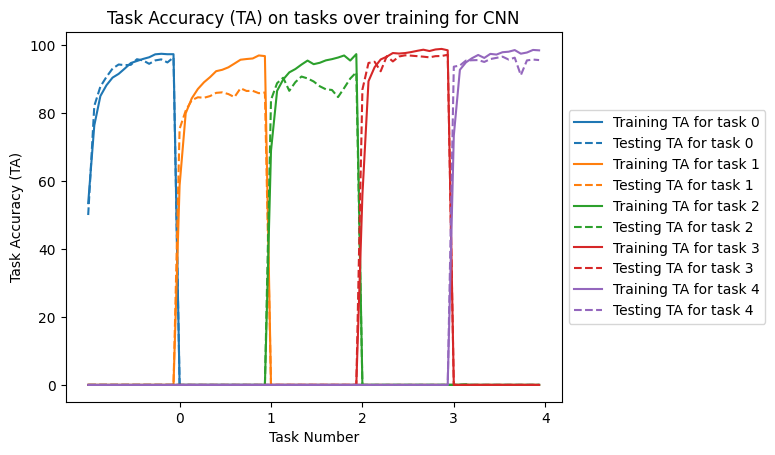
\includegraphics[width=\linewidth]{images/CIFAR10_CL/CNN_TA_task.png}
       \caption{All the TA's for CNN over training, it achieves at least 86\% testing CTA by the end of training on each task. Note that learning on new tasks appears more gradual with this network. Complete forgetting happens instantly for all tasks.}
    \end{subfigure}
    \quad % add space between images
    \begin{subfigure}[t]{0.4\textwidth}
       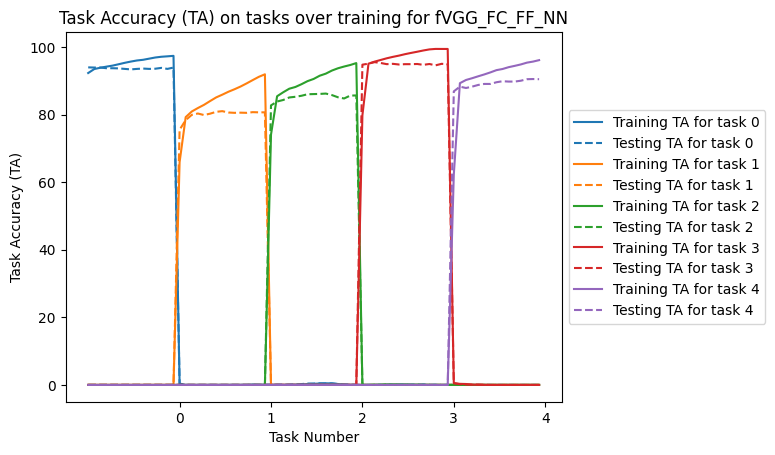
\includegraphics[width=\linewidth]{images/CIFAR10_CL/fVGG_FC_FF_NN_TA_task.png}
       \caption{All the TA's for the fVGG-FCFFNN over training, it achieves at least 80\% testing CTA by the end of training on each task. Complete forgetting happens instantly for all tasks.}
    \end{subfigure}
    
    \medskip % add space between rows
    
    \begin{subfigure}[t]{0.4\textwidth}
       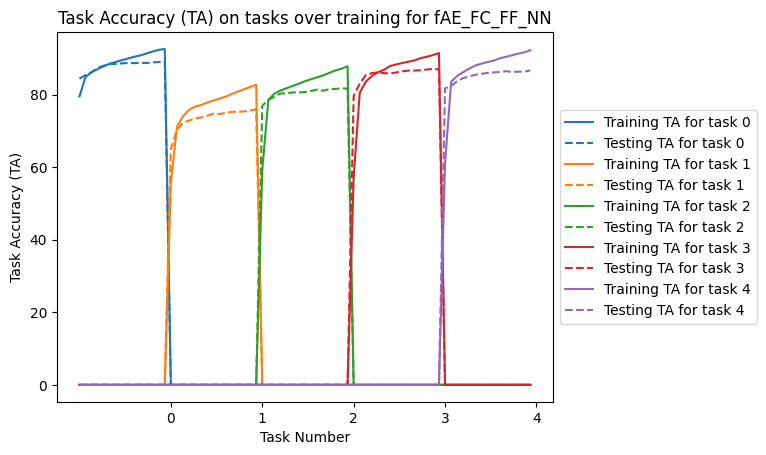
\includegraphics[width=\linewidth]{images/CIFAR10_CL/fAE_FC_FF_NN_TA_task.png}
       \caption{All the TA's for the fAE-FCFFNN over training, it achieves at least 75\% testing CTA by the end of training on each task, which is a fair bit less than what the other networks were able to achieve. Complete forgetting happens instantly for all tasks.}
    \end{subfigure}
    \quad % add space between images
    \begin{subfigure}[t]{0.4\textwidth}
       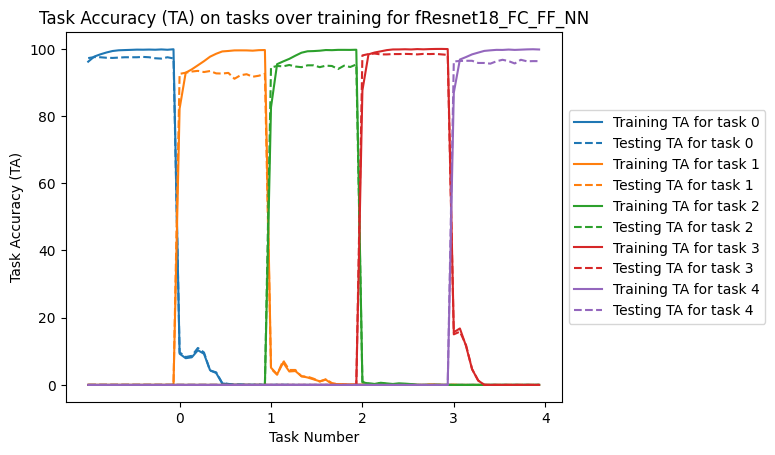
\includegraphics[width=\linewidth]{images/CIFAR10_CL/fResnet18_FC_FF_NN_TA_task.png}
       \caption{All the TA's for fResnet18-FCFFNN over training, it achieves at least 94\% testing CTA by the end of training on each task. Forgetting is again very evident, however, unlike other networks for some tasks it takes some time before the TA for the previous task drops to zero.}
    \end{subfigure}

    \medskip % add space between rows

    \begin{subfigure}[t]{0.4\textwidth}
      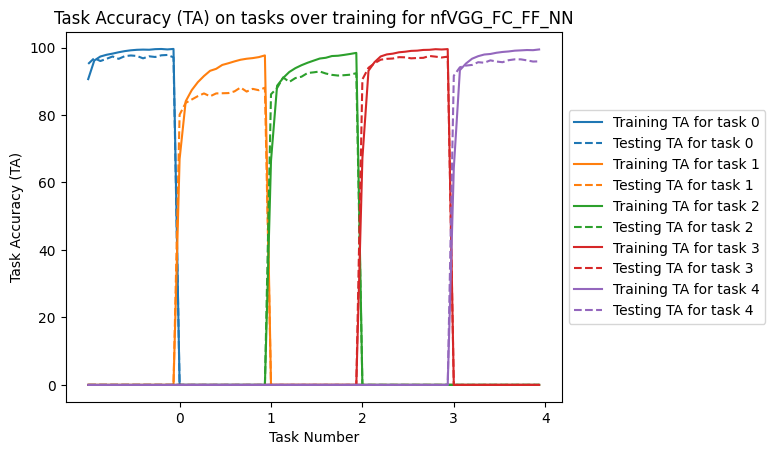
\includegraphics[width=\linewidth]{images/CIFAR10_CL/nfVGG_FC_FF_NN_TA_task.png}
      \caption{All the TA's for nfVGG-FCFFNN over training, it achieves at least 88\% testing CTA by the end of training on each task. Complete forgetting happens instantly for all tasks.}
   \end{subfigure}
   \quad % add space between images
   \begin{subfigure}[t]{0.4\textwidth}
      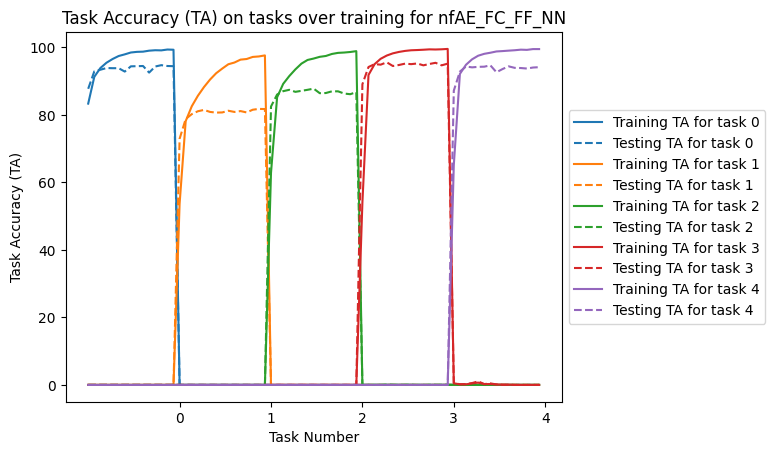
\includegraphics[width=\linewidth]{images/CIFAR10_CL/nfAE_FC_FF_NN_TA_task.png}
      \caption{All the TA's for nfAE-FCFFNN over training, it achieves at least 81\% testing CTA by the end of training on each task. Again forgetting here is immediate and catastrophic.}
   \end{subfigure}

    \medskip % add space between rows

    \begin{subfigure}[t]{0.4\textwidth}
      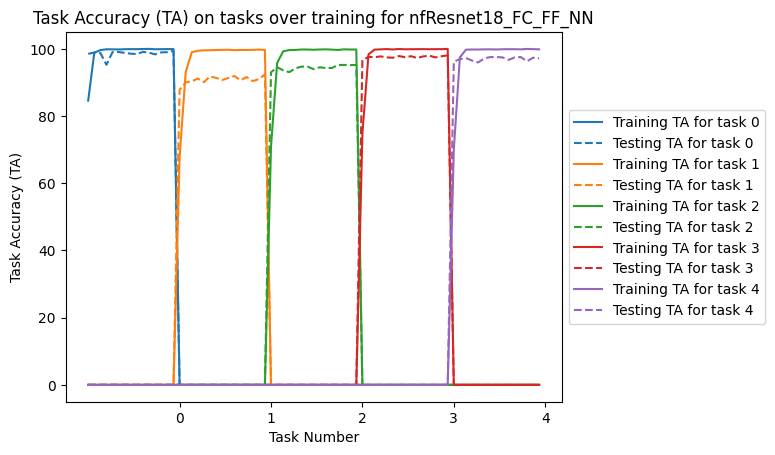
\includegraphics[width=\linewidth]{images/CIFAR10_CL/nfResnet18_FC_FF_NN_TA_task.png}
      \caption{All the TA's for nfResnet18-FCFFNN over training, it achieves at least 92\% testing CTA by the end of training on each task, which is second only to it's frozen counterpart. However, unlike it's frozen counterpart forgetting is immediate and catastrophic.}
   \end{subfigure}
    
    \caption{The testing and training TA's on each individual task over training epochs for all the networks we trained on split-CIFAR10. fResnet18-FCFFNN got the best performance in terms of CTA and was the only network to not forget all previous task knowledge straight after training on a new task.}
    \label{fig:CIFAR10-CL-TA}
\end{figure}
% \FloatBarrier

\begin{table}[ht]
    \centering
    \begin{tabular}{l c c}
    \toprule
    \textbf{Model Name} & \textbf{Total compute time (seconds)} & \textbf{Total Trainable Parameters} \\
    \midrule
    \textbf{CNN} & 20218.98 & 15245130 \\
    \textbf{fVGG-FCFFNN} & 6181.29 & 530442 \\
    \textbf{nfVGG-FCFFNN} & 22893.2 & 15253578 \\
    \textbf{fAE-FCFFNN} & 5319.08 & \textbf{399370} \\
    \textbf{nfAE-FCFFNN} & 8315.19 & 685354 \\
    \textbf{fResnet18-FCFFNN} & \textbf{5502.08} & 530442 \\
    \textbf{nfResnet18-FCFFNN} & 31487.58 & 11706954 \\
    \bottomrule
    \end{tabular}
    \caption{Table of compute times and total number of trainable parameters of our models trained on split-CIFAR10, one NVIDIA GeForce RTX 2080 Ti was used to train each of these models.}
    \label{tab:compute_times}
\end{table}

\begin{figure}[ht]
  \centering
  \begin{subfigure}[t]{0.4\textwidth}
     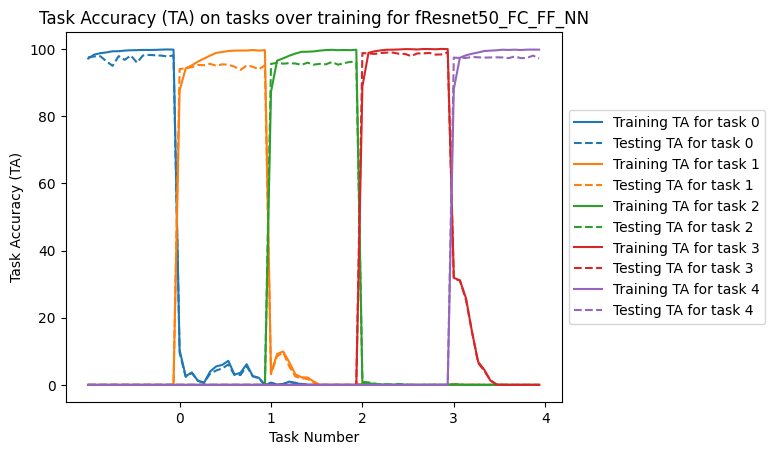
\includegraphics[width=\linewidth]{images/CIFAR10_CL/fResnet50_FC_FF_NN_TA_task.png}
     \caption{The TA's for fResnet50-FCFFNN over training. We see for every task (bar task 2) that forgetting is more gradual with it being especially pronounced for task 0 where complete forgetting only seems to occur right at the end of training on task 0.}
  \end{subfigure}
  \quad % add space between images
  \begin{subfigure}[t]{0.4\textwidth}
     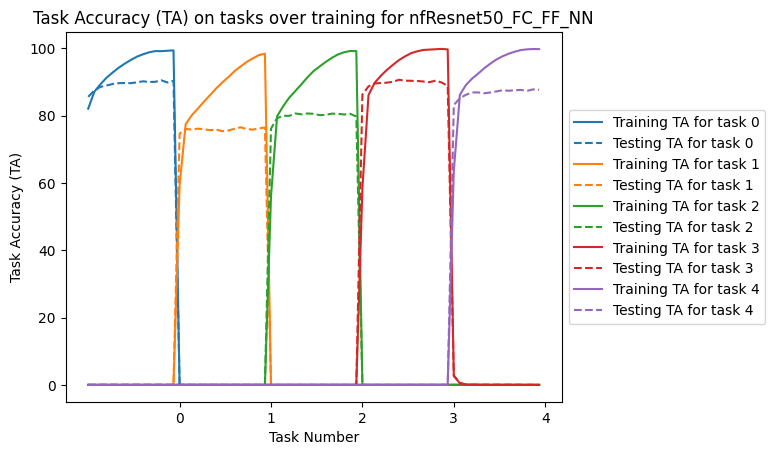
\includegraphics[width=\linewidth]{images/CIFAR10_CL/nfResnet50_FC_FF_NN_TA_task.png}
     \caption{The TA's for nfResnet50-FCFFNN over training. Here weo observe complete forgetting as soon as we begin training on the next task.}
  \end{subfigure}

  \caption{The testing and training TA's on each individual task over training epochs for networks with Resnet50 used for the encoder on split-CIFAR10. We observe some more gradual forgetting in the network that has the frozen encoder, however, the non-frozen network displays quick complete forgetting of the previous task.}
  \label{fig:CIFAR10-R50-TA}
\end{figure}

\FloatBarrier
\subsection{Investigating the effect of resetting on CF}
\label{sec:resetting}
We also carried out a series of experiments where we reset the fully connected classifier portion of the network, ie. randomly initialize the weights, at the end of each task. We ran the same networks as in \cref{sec:pretrain-freeze} on split-CIFAR10 and again kept tab on their loss and accuracy on testing and training data individually for each task aswell as the time needed for compute. We carried out these experiments to evaluate how the performance of training with a random classifier head compares to training with a classifier head that's been trained on previous tasks. \Cref{fig:CIFAR10-CL-TA-reset} shows the TA's over training, we observe extremely similar results to the networks without reset, except for with fResnet18-FCFFNN where the TA's of some tasks don't gradually reduce (which makes sense as we are randomly scrambling the weights). 

Using these results we suggest a novel CL technique, where we create a classifier head for each task. From our results it appears a method that uses a newly randomly initialized classifier for each task achieves performance very similar to networks where the classifier head has trained on other tasks and with the same amount of forgetting (in most cases) due to the severity of forgetting we have seen in our experiments. If we simply trained and kept a small classifier head for each task then we would be able to achieve the same level of CTA as without reset except we would have no forgetting as the classifier head only ever has trained on one task. This somewhat bypasses the problem of CF and seems like a potentially good naive method for CL. The obvious downsides of such a method being that we need to have knowledge of what task we are currently training on and we must create a new classifier head for each task. It's also not clear whether such a method might hold up in more complex problem settings. Plots showing the TL over training and compute times for training the networks with reset are available in \cref{sec:resetting-TL}.

\begin{figure}[ht]
  \centering
  \begin{subfigure}[t]{0.4\textwidth}
     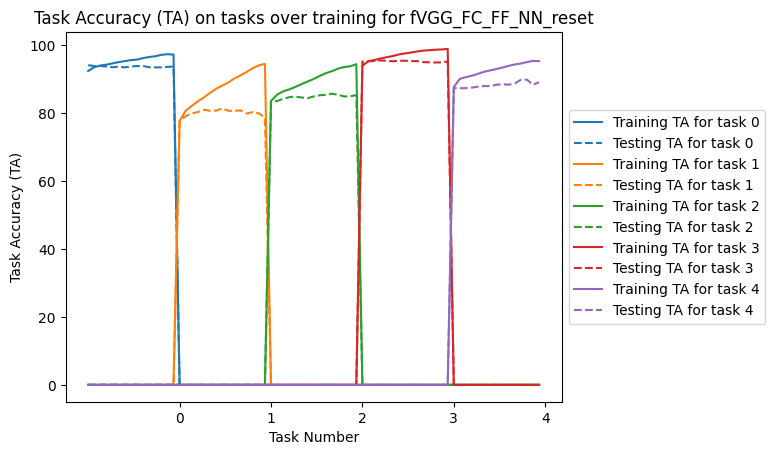
\includegraphics[width=\linewidth]{images/CIFAR10_CL/fVGG_FC_FF_NN_reset_TA_task.png}
     \caption{All the TA's for the fVGG-FCFFNN with reset over training, it's results mirror extremely closely the results of the fVGG-FCFFNN without reset.}
  \end{subfigure}
  \quad
  \begin{subfigure}[t]{0.4\textwidth}
     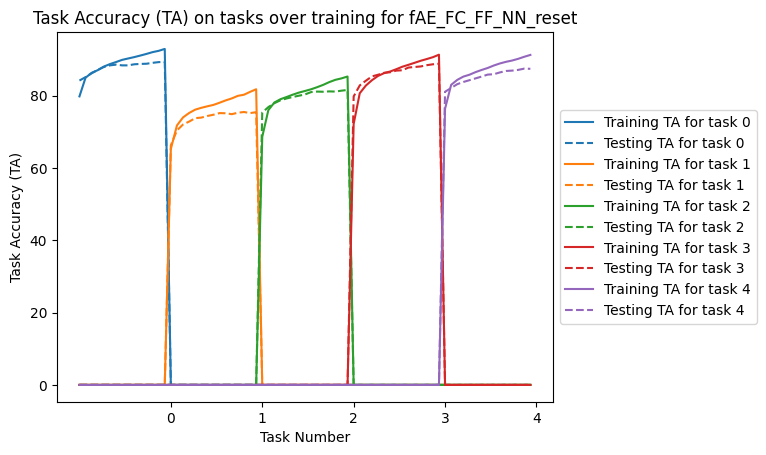
\includegraphics[width=\linewidth]{images/CIFAR10_CL/fAE_FC_FF_NN_reset_TA_task.png}
     \caption{All the TA's for the fAE-FCFFNN with reset over training, it's results mirror extremely closely the results of this network without reset.}
  \end{subfigure}
  
  \medskip % add space between rows

  \begin{subfigure}[t]{0.4\textwidth}
     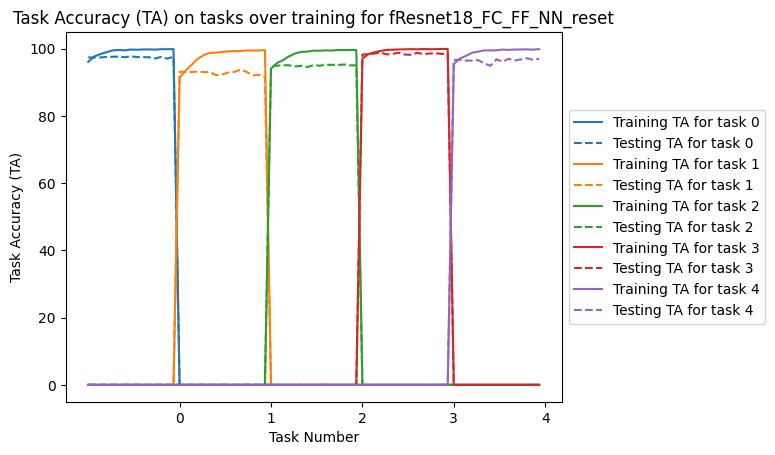
\includegraphics[width=\linewidth]{images/CIFAR10_CL/fResnet18_FC_FF_NN_reset_TA_task.png}
     \caption{All the TA's for fResnet18-FCFFNN with reset over training, it achieves very similar results to the fResnet18-FCFFNN without reset. Except with reset the more gradual forgetting isn't witnessed (as would be expected randomly initializing the head of the network).}
  \end{subfigure}
  \quad
  \begin{subfigure}[t]{0.4\textwidth}
    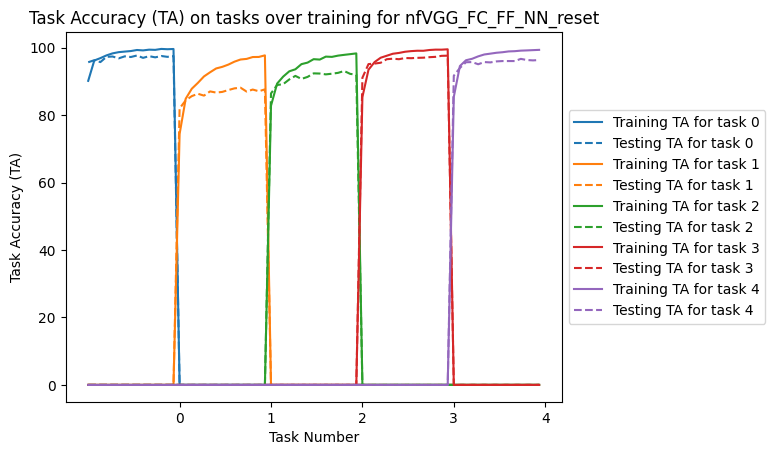
\includegraphics[width=\linewidth]{images/CIFAR10_CL/nfVGG_FC_FF_NN_reset_TA_task.png}
    \caption{All the TA's for nfVGG-FCFFNN with reset over training, it's results closely resemble the results of this network without reset.}
 \end{subfigure}
 
 \medskip % add space between rows

 \begin{subfigure}[t]{0.4\textwidth}
    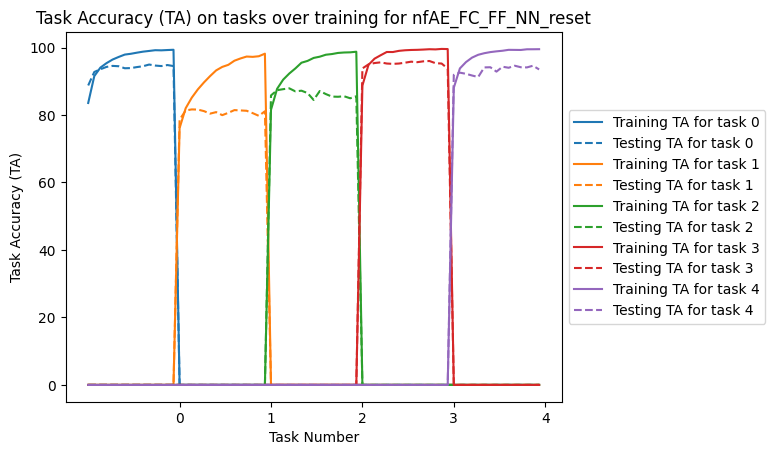
\includegraphics[width=\linewidth]{images/CIFAR10_CL/nfAE_FC_FF_NN_reset_TA_task.png}
    \caption{All the TA's for nfAE-FCFFNN with reset over training, it's results also closely resemble the results without reset, except for a slightly more gradual learning curve when it's just started training on a new task.}
 \end{subfigure}
 \quad
  \begin{subfigure}[t]{0.4\textwidth}
    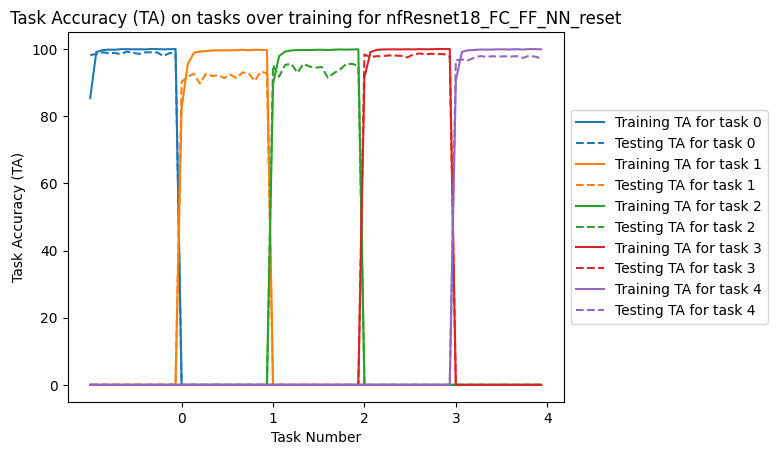
\includegraphics[width=\linewidth]{images/CIFAR10_CL/nfResnet18_FC_FF_NN_reset_TA_task.png}
    \caption{All the TA's for nfResnet18-FCFFNN with reset over training, it's results also closely resemble the results of this network without reset.}
 \end{subfigure}
  
  \caption{The testing and training TA's on each individual task over training epochs for all the networks we trained on split-CIFAR10. All the results here are extremely similar to the results in \cref{fig:CIFAR10-CL-TA} without reset, although the results for fResnet18-FCFFNN do differ slightly.}
  \label{fig:CIFAR10-CL-TA-reset}
\end{figure}